% ============================================================
% Lecture 2 -- Data Visualization using ggplot2
% ============================================================
\section{Data Visualization using ggplot2}\label{sec:L02}

\lectureheader{2}{7nmwfGpgDkM}{Week-1 slides \texttt{Jan26notes.pdf}, ggplot2 part (slides on aesthetics, scaling, viridis, facets)}

\begin{guiding*}
By the end of this lecture you should be able to:
\begin{itemize}
  \item explain the idea of a \emph{grammar of graphics} and the basic \texttt{ggplot} template;
  \item map a variable to an \emph{aesthetic} (colour, shape, size) and explain what \emph{scaling} does;
  \item use colour-blind-safe \emph{viridis} palettes;
  \item split a plot into \emph{facets} with \texttt{facet\_wrap} and \texttt{facet\_grid};
  \item reproduce all of these plots in Python with \texttt{seaborn}/\texttt{matplotlib}.
\end{itemize}
\end{guiding*}

\subsection{Recap and motivation}
In \cref{sec:L01} we used R's base graphics (\texttt{hist}, \texttt{plot}). They are quick, but
each kind of plot has its own function with its own arguments. The package \texttt{ggplot2}
(loaded by \texttt{library(tidyverse)}) takes a different route: it is built on a \emph{grammar
of graphics}. The instructor's annotation sums up the benefit: ``a system for describing and
building graphs --- learn one system and apply it at many places''. In linear models we
constantly plot a response against predictors, coloured or split by a factor. This is exactly
what the grammar makes easy.

\subsection{The \texttt{mpg} data}
The running example is the tidyverse data set \texttt{mpg}. It contains observations collected
by the US Environmental Protection Agency on $38$ models of cars ($234$ rows, $11$ columns).
Two variables matter most here:
\begin{itemize}
  \item \texttt{displ}: engine displacement in litres (the car's engine size);
  \item \texttt{hwy}: fuel efficiency on the highway, in miles per gallon.
\end{itemize}
Other variables used below are \texttt{class} (type of car: 2seater, compact, midsize, minivan,
pickup, subcompact, suv), \texttt{drv} (\texttt{f} = front-wheel, \texttt{r} = rear-wheel,
\texttt{4} = four-wheel drive), \texttt{cyl} (number of cylinders) and \texttt{trans} (type of
transmission).

\subsection{The basic template}
The first plot on the slides is
\codeline{ggplot(data = mpg) + geom\_point(mapping = aes(x = displ, y = hwy))}
It shows a \emph{negative relationship between engine size and fuel efficiency}: cars with big
engines use more fuel.

\begin{definition}[The ggplot template]\label{def:L02-template}
A \texttt{ggplot2} graph is built in layers:
\begin{enumerate}
  \item \texttt{ggplot(data = <DATA>)} creates a coordinate system to which layers are added. On its own it draws an empty graph.
  \item A \vocab{geom function} such as \texttt{geom\_point()} adds a layer, here a layer of points.
  \item Each geom takes a \texttt{mapping} argument, which is always paired with \texttt{aes()}. It says which variables go on which visual channels.
\end{enumerate}
In short: \texttt{ggplot(data = <DATA>) + <GEOM\_FUNCTION>(mapping = aes(<MAPPINGS>))}.
\end{definition}

\subsection{Aesthetic mappings and scaling}
\begin{definition}[Aesthetic, mapping, scaling]\label{def:L02-aes}
An \vocab{aesthetic} is a visual property of the objects in the plot: position ($x$, $y$),
\texttt{colour}, \texttt{shape}, \texttt{size}, and so on. To \vocab{map} a variable to an
aesthetic we associate the aesthetic's name with the variable's name inside \texttt{aes()}.
\vocab{Scaling} is the step in which \texttt{ggplot2} assigns a unique level of the aesthetic
(a colour, say) to each unique level of the variable. It also adds a legend that explains the
correspondence.
\end{definition}

\begin{example}[Adding a third variable]\label{ex:L02-colour}
\texttt{ggplot(data=mpg) + geom\_point(mapping=aes(x=displ, y=hwy, colour=class))} adds the
variable \texttt{class} to the two-dimensional scatter plot by mapping it to the aesthetic
\texttt{colour}. Here the aesthetic's name is \texttt{colour} and the variable is
\texttt{class}. Scaling assigns $7$ colours to the $7$ classes, and the legend lists them.
The plot shows that most of the cars with large engines but unusually \emph{good} mileage are
\texttt{2seater}s. These are sports cars: big engines, but light bodies.
\end{example}
Other aesthetics include \texttt{shape} and \texttt{size}. The instructor notes on the slide
that one can add \texttt{shape} in exactly the same way.

\begin{figure}[ht]
\centering
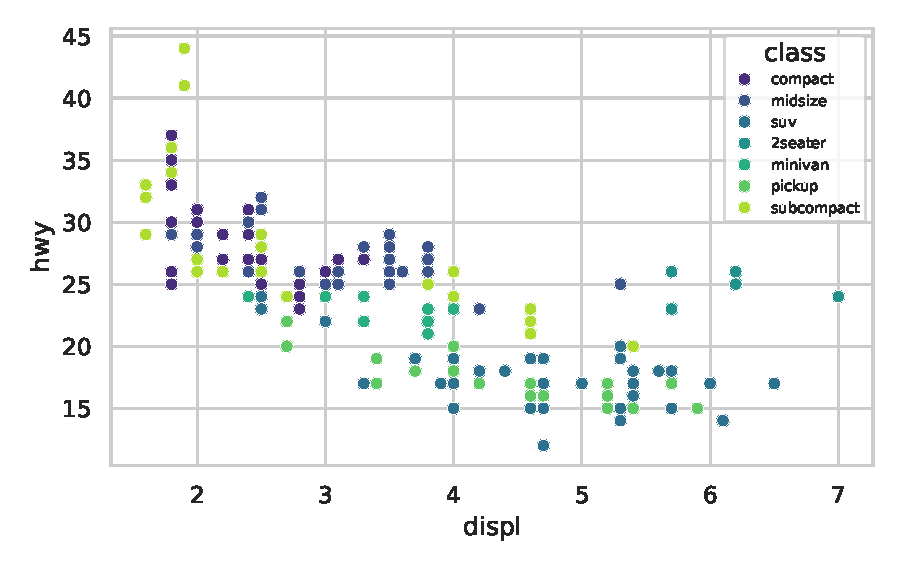
\includegraphics[width=0.7\textwidth]{figures/L02_mpg_class.pdf}
\caption{\texttt{hwy} against \texttt{displ}, coloured by \texttt{class} (viridis palette).}
\label{fig:L02-class}
\end{figure}

\begin{note}[Supplementary: mapping versus setting]
Putting \texttt{colour = class} \emph{inside} \texttt{aes()} maps a variable to colour. Putting
\texttt{colour = "blue"} \emph{outside} \texttt{aes()} just sets every point to blue. A common
beginner's mistake is \texttt{aes(colour = "blue")}. This maps a constant \emph{variable} whose
single level is the string \texttt{"blue"}, so the points get the first default colour
(pinkish-red) and a pointless legend appears.
\end{note}

\subsection{Viridis colour scales}
The viridis scales give colour maps that are \emph{perceptually uniform} in both colour and
black-and-white. They are also designed to be read correctly by viewers with common forms of
colour blindness (see \url{https://bids.github.io/colormap/}). Adding
\texttt{+ scale\_colour\_viridis\_d()} to the previous plot switches to the default viridis
palette for a discrete variable. \texttt{scale\_colour\_viridis\_d(option = "plasma")} chooses
the ``plasma'' variant.

\subsection{Facets}
Aesthetics are one way to add a variable. Another, especially useful for categorical variables,
is to split the plot into \vocab{facets}.

\begin{definition}[Facets]\label{def:L02-facets}
\texttt{facet\_wrap(\textasciitilde\ class, nrow = 2)} splits a plot by a \emph{single} variable
into subplots, each showing one subset of the data. \texttt{facet\_grid(drv \textasciitilde\ cyl)}
splits by the \emph{combination} of two variables: rows are levels of \texttt{drv}, columns are
levels of \texttt{cyl}.
\end{definition}

\begin{example}[Facets on \texttt{mpg}]\label{ex:L02-facets}
With \texttt{facet\_wrap(\textasciitilde class, nrow=2)} we get seven panels. The pickup and SUV
panels show large engines and low mileage, while the compact and subcompact panels contain the
high-mileage cars. With \texttt{facet\_grid(drv\textasciitilde cyl)} the $3\times 4$ grid shows,
for instance, that there are \emph{no} rear-wheel-drive cars with $4$ or $5$ cylinders in the
data. Those cells are empty. Facets and colour can be combined, as on the last slide of this
part:
\texttt{geom\_point(aes(colour=class)) + scale\_colour\_viridis\_d(option="plasma") + facet\_wrap(\textasciitilde class, nrow=2)}.
\end{example}

\begin{figure}[ht]
\centering
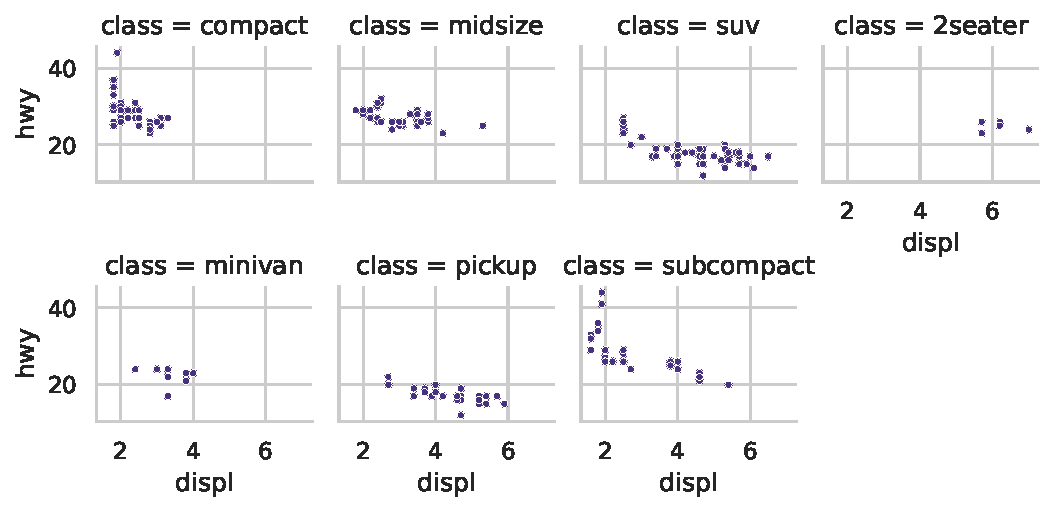
\includegraphics[width=0.95\textwidth]{figures/L02_mpg_facets.pdf}
\caption{\texttt{facet\_wrap(\textasciitilde\ class)}: one panel per class.}
\label{fig:L02-facets}
\end{figure}

\begin{note}[Supplementary: why facets matter for linear models]
In a regression of \texttt{hwy} on \texttt{displ}, the relationship could differ between
classes. For example, the slope within SUVs could differ from the slope within compacts.
Faceting by a factor is the visual version of fitting a model with a
\emph{factor $\times$ covariate interaction}. That is the analysis of covariance (ANCOVA), which
comes later in the course.
\end{note}

\subsection{Computation}
\begin{center}
\small\begin{tabular}{@{}>{\raggedright\arraybackslash}p{7.3cm}>{\raggedright\arraybackslash}p{8.3cm}@{}}\hline
R (\texttt{ggplot2}) & Python (\texttt{seaborn})\\\hline
\texttt{ggplot(mpg)+geom\_point(aes(displ,hwy))} & \texttt{sns.scatterplot(data=mpg, x="displ", y="hwy")}\\
\texttt{aes(..., colour=class)} & \texttt{hue="class"}\\
\texttt{scale\_colour\_viridis\_d()} & \texttt{palette="viridis"}\\
\texttt{option="plasma"} & \texttt{palette="plasma"}\\
\texttt{facet\_wrap(\textasciitilde class, nrow=2)} & \texttt{sns.relplot(..., col="class", col\_wrap=4)}\\
\texttt{facet\_grid(drv\textasciitilde cyl)} & \texttt{sns.relplot(..., row="drv", col="cyl")}\\\hline
\end{tabular}
\end{center}
See \nb{week01/L02\_ggplot2.ipynb}.

\subsection{Summary}
\begin{itemize}
  \item Template: \texttt{ggplot(data) + geom(mapping = aes(...))}.
  \item Aesthetics (colour, shape, size) add variables. Scaling turns variable levels into aesthetic levels and makes a legend.
  \item Viridis palettes are perceptually uniform and colour-blind safe.
  \item \texttt{facet\_wrap} splits by one variable; \texttt{facet\_grid} by two.
  \item \texttt{mpg}: engine size and highway mileage are negatively related, and the 2-seaters are the exception.
\end{itemize}

\subsection{Exercises}
\begin{problem}\label{prob:L02-1}
What goes wrong with \texttt{ggplot(mpg) + geom\_point(aes(displ, hwy, colour = "blue"))}? How do you make all points blue?
\end{problem}
\begin{problem}\label{prob:L02-2}
Map the continuous variable \texttt{cty} to \texttt{colour}. How does the legend differ from the one for \texttt{class}? Do the same in seaborn.
\end{problem}
\begin{problem}\label{prob:L02-3}
Using \texttt{facet\_grid(drv \textasciitilde\ cyl)} (or its seaborn equivalent), list the empty cells. What do they tell you about the cars in the data?
\end{problem}
\begin{problem}\label{prob:L02-4}
Count how many distinct values \texttt{class}, \texttt{drv} and \texttt{cyl} take in \texttt{mpg}. How many panels does \texttt{facet\_grid(drv \textasciitilde\ cyl)} have?
\end{problem}

\subsection{Further reading}
Wickham \& Grolemund, \emph{R for Data Science}, Chapter~3 (Data visualisation) --- the source
the instructor follows. Christensen and Rao do not cover graphics. Christensen's regression
chapters (Chapter~6 onwards) use residual plots of the kind built with these tools.
